\documentclass[12pt]{article}
\usepackage[left=1cm, right=1cm, top=2cm,bottom=1.5cm]{geometry} 

\usepackage[parfill]{parskip}
\usepackage[utf8]{inputenc}
\usepackage[T2A]{fontenc}
\usepackage[russian]{babel}
\usepackage{enumitem}
\usepackage[normalem]{ulem}
\usepackage{amsfonts, amsmath, amsthm, amssymb, mathtools}
\usepackage{tabularx}
\usepackage{hhline}

\usepackage{accents}
\usepackage{fancyhdr}
\pagestyle{fancy}
\renewcommand{\headrulewidth}{1.5pt}
\renewcommand{\footrulewidth}{1pt}

\usepackage{graphicx}
\usepackage[figurename=Рис.]{caption}
\usepackage{subcaption}
\usepackage{float}

%%Наименование папки откуда забирать изображения
\graphicspath{ {./images/} }

%%Изменение формата для ввода доказательства
\renewcommand{\proofname}{$\square$  \nopunct}
\renewcommand\qedsymbol{$\blacksquare$}

%%Изменение отступа на таблицах
\addto\captionsrussian{%
	\renewcommand{\proofname}{$\square$ \nopunct}%
}
%% Римские цифры
\newcommand{\RN}[1]{%
	\textup{\uppercase\expandafter{\romannumeral#1}}%
}

%% Для удобства записи
\newcommand{\MR}{\mathbb{R}}
\newcommand{\MQ}{\mathbb{Q}}
\newcommand{\MN}{\mathbb{N}}
\newcommand{\MI}{\mathrm{I}}
\newcommand{\MJ}{\mathrm{J}}
\newcommand{\MH}{\mathrm{H}}
\newcommand{\MT}{\mathrm{T}}
\newcommand{\MU}{\mathcal{U}}
\newcommand{\MV}{\mathcal{V}}
\newcommand{\VN}{\varnothing}
\newcommand{\VE}{\varepsilon}

\theoremstyle{definition}
\newtheorem{defn}{Опр:}
\newtheorem{rem}{Rm:}
\newtheorem{prop}{Утв.}
\newtheorem{exrc}{Упр.}
\newtheorem{lemma}{Лемма}
\newtheorem{theorem}{Теорема}
\newtheorem{corollary}{Следствие}

\newenvironment{cusdefn}[1]
{\renewcommand\thedefn{#1}\defn}
{\enddefn}

\DeclareRobustCommand{\divby}{%
	\mathrel{\text{\vbox{\baselineskip.65ex\lineskiplimit0pt\hbox{.}\hbox{.}\hbox{.}}}}%
}
%Короткий минус
\DeclareMathSymbol{\SMN}{\mathbin}{AMSa}{"39}
%Длинная шапка
\newcommand{\overbar}[1]{\mkern 1.5mu\overline{\mkern-1.5mu#1\mkern-1.5mu}\mkern 1.5mu}
%Функция знака
\DeclareMathOperator{\sgn}{sgn}

%Обозначение константы
\DeclareMathOperator{\const}{\text{const}}

%Интеграл в большом формате
\DeclareMathOperator{\dint}{\displaystyle\int}

\newcommand{\smallerrel}[1]{\mathrel{\mathpalette\smallerrelaux{#1}}}
\newcommand{\smallerrelaux}[2]{\raisebox{.1ex}{\scalebox{.75}{$#1#2$}}}

\newcommand{\smallin}{\smallerrel{\in}}
\newcommand{\smallnotin}{\smallerrel{\notin}}

\newcommand*{\medcap}{\mathbin{\scalebox{1.25}{\ensuremath{\cap}}}}%
\newcommand*{\medcup}{\mathbin{\scalebox{1.25}{\ensuremath{\cup}}}}%

%Скалярное произведение
\DeclarePairedDelimiterX{\inner}[2]{\langle}{\rangle}{#1, #2}

%Подпись символов снизу
\newcommand{\ubar}[1]{\underaccent{\bar}{#1}}

\begin{document}
\lhead{Математический анализ - \RN{2}}
\chead{Шапошников С.В.}
\rhead{Лекция - 10}
\section*{Непрерывность функций}
Пусть $(X,\rho_X)$ и $(Y,\rho_Y)$ - метрические пространства, $a \in X$. Пусть $f\colon X \to Y$.
\begin{defn}
	Функция $f$ \uwave{непрерывна в точке} $a \in X$, если
	$$
	\forall \VE > 0, \, \exists \, \delta > 0 \colon \rho_X(x,a) < \delta \Rightarrow \rho_Y(f(x),f(a)) < \VE
	$$
\end{defn}

\begin{theorem}
	Следующие утверждения равносильны:
	\begin{enumerate}[label ={(\arabic*)}]
		\item $f$ - непрерывна в точке $a$;
		\item $\forall \{x_n\} \in X,\,  x_n \to a \Rightarrow f(x_n) \to f(a)$;
		\item Или $a$ - это изолированная точка, или $a$ - это предельная точка $X$ и $\lim\limits_{x \to a} f(x) = f(a)$;
	\end{enumerate}
\end{theorem}

Пусть $f \colon \MR^2 \to \MR$. Пусть $a = (a_1,a_2)$, $\rho_X(x,y) = \sqrt{(x_1 - y_1)^2 + (x_2 - y_2)^2}$ - стандартная Евклидова метрика, $\rho_Y(u,v) = |u - v|$. Тогда, $f$ непрерывна в точке $a$ будет обозначать, что:
$$
	\forall \VE > 0, \, \exists \, \delta > 0 \colon \sqrt{(x_1 - a_1)^2 + (x_2 - a_2)^2} < \delta \Rightarrow |f(x_1,x_2) - f(a_1,a_1) | < \VE
$$
Исходя из того, что
\begin{itemize}
	\item $x \to f(x,y)$ - непрерывна в точке $a_1, \, \forall y$;
	\item $y \to f(x,y)$ - непрерывна в точке $a_2, \, \forall x$;
\end{itemize}
можно ли сделать вывод что $f$ непрерывна в точке $(a_1,a_2)$?

В данном случае, функция непрерывна вдоль горизонтальных и вертикальных прямых.
\begin{figure}[H]
	\centering
	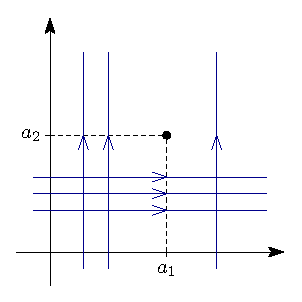
\includegraphics[width=0.3\textwidth]{10_1.eps}
	\caption{Функция непрерывна в точке $(a_1,a_2)$ по каждой из переменных.}
	\label{10_1}
\end{figure}
В заданном нами определении, функция может подходить к проверяемой точке каким угодно способом. Поэтому если функция непрерывна по каждой из переменных, то это не означает, что она непрерывна в точке $(a_1,a_2)$.

\textbf{Пример}: Возьмем точку $a = (a_1, a_2) = (0,0)$. Рассмотрим функцию $f(x_1,x_2) = \begin{cases} 1, & x_2 = x_1^2 \wedge x_1 \geq 0 \\ 0, & x_2 \neq x_1^2 \vee x_1 < 0 \end{cases}$.
\begin{figure}[H]
	\centering
	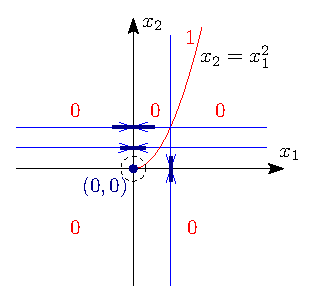
\includegraphics[width=0.3\textwidth]{10_2.eps}
	\caption{Функция непрерывна в точке $(0,0)$ по каждой из переменных, но разрывная в $(0,0)$.}
	\label{10_2}
\end{figure}
Эта функция непрерывна по каждой из переменных в точке $(0,0)$: 

При подходе к $x_2 = 0$ она в целой окрестности будет тождественным нулем. Чем ближе к $x_2 = 0$, тем меньше окрестность, но в ней функция все равно будет тождественно нулевая, а при $x_2 = 0$ функция $f(x_1,0) \equiv 0$.

При подходе к $x_1 = 0$ ситуация аналогичная. Функция в целой окрестности будет тождественным нулем. Чем ближе к $x_1 = 0$, тем меньше окрестность, но в ней функция все равно будет тождественно нулевая, а при $x_1 = 0$ функция $f(0,x_2) \equiv 0$.

Но при всем этом, эта функция не является непрерывной в точке $(0,0)$, поскольку как бы близко не взяли точку к началу координат, там будет значение функции $0$ и значение функции $1$:
$$
	\forall\, 1 > \VE > 0, \, \nexists \, \delta > 0 \colon \sqrt{(x_1 - a_1)^2 + (x_2 - a_2)^2} < \delta \Rightarrow |f(x_1,x_2) - f(a_1,a_1) | < \VE
$$
Чего не хватает, чтобы функция была непрерывной по совокупности переменных? \\
Рассмотрим следующее неравенство:
$$
	|f(x_1,x_2) - f(a_1,a_2)|\leq |f(x_1,x_2) - f(a_1, x_2)| + |f(a_1,x_2) - f(a_1,a_2)|
$$
Выбираем $\delta$ для первого слагаемого, начинаем выбирать $\delta$ для второго, тогда $x_2$ начнет приближаться к $a_2$ и тем самым $\delta$ в первом слагаемом могло испортиться. Такой эффект возникает поскольку не хватает равномерности.

\begin{prop}
	Пусть $x_1 \to f(x_1,x_2)$ - непрерывна в точке $a_1$ равномерно по $x_2$, то есть:
	$$
		\sup\limits_{x_2}|f(x_1,x_2) - f(a_1,x_2)| \xrightarrow[x_1 \to a_1]{} 0
	$$
	или по-другому $f(x_1,x_2)\overset{x_2}{\underset{x_1 \to a_1}{\rightrightarrows}} f(a_1,x_2)$. Пусть $x_2 \to f(x_1,x_2)$ - непрерывна в точке $a_2$. Тогда $f$ - непрерывна в точке $(a_1,a_2)$. 
\end{prop}
\begin{proof}
	Рассмотрим неравенство $|f(x_1,x_2) - f(a_1,a_2)|\leq |f(x_1,x_2) - f(a_1, x_2)| + |f(a_1,x_2) - f(a_1,a_2)|$, тогда:
	$$
		|f(x_1,x_2) - f(a_1, x_2)| + |f(a_1,x_2) - f(a_1,a_2)| \leq \sup\limits_{x_2}|f(x_1,x_2) - f(a_1,x_2)| + |f(a_1,x_2) - f(a_1,a_2)|
	$$
	Пусть задан $\VE > 0$, найдем $\delta > 0$:
	$$
		|x_1 - a_1| < \delta \Rightarrow \sup\limits_{x_2}|f(x_1,x_2) - f(a_1,x_2)| < \VE
	$$
	$$
		|x_2 - a_2| < \delta \Rightarrow |f(a_1,x_2) - f(a_1,a_2)| < \VE
	$$ 
	
	Тогда, если $\rho_X(x,a) = \sqrt{(x_1 - a_1)^2 + (x_2 - a_2)^2} < \delta$, то $|x_1 - a_1| < \delta \wedge |x_2 - a_2| < \delta$, следовательно :
	$$
		|f(x_1,x_2) - f(a_1,a_2)| \leq \sup\limits_{x_2}|f(x_1,x_2) - f(a_1,x_2)| + |f(a_1,x_2) - f(a_1,a_2)| <  \VE + \VE = 2\VE
	$$
\end{proof}
\begin{rem}
	Если функция непрерывна в любой точке по каждой переменной в отдельности, то из этого следует, что непрерывность по совокупности не пропадает вовсе.
\end{rem}

\begin{prop}
	Пусть $(X,\rho)$ - метрическое пространство, $(Y,\| \cdot \|)$ - нормированное пространство ($\rho_Y = \| \cdot \|$). Пусть $f, g \colon X \to Y, \, \alpha \colon X \to \MR$ - непрерывны в точке $a$, тогда $f + g$ и $\alpha{\cdot}f$ - непрерывны в точке $a$.
\end{prop}
\begin{proof}
	Пусть $x_n \to a \Rightarrow f(x_n) \to f(a),\, g(x_n) \to g(a), \, \alpha(x_n) \to \alpha(a)$. Все следует из свойств предела последовательности для нормированных пространств.
\end{proof}

\begin{prop}
	Пусть $(X,\rho_X),\, (Y,\rho_Y), \, (Z,\rho_Z) $ - метрические пространства. $f\colon X \to Y, \, g \colon Y \to Z$. Если $f$ непрерывна в точке $a$ и $g$ непрерывна в точке $f(a)$, то $g(f)$ - непрерывна в точке $a$.
\end{prop}
\begin{proof}
	Пусть $x_n \to a \Rightarrow f(x_n) \to f(a)\Rightarrow g(f(x_n)) \to g(f(a))$.
\end{proof}

\begin{defn}
	Функция $f \colon X \to Y$ \uwave{непрерывна}, если $f$ непрерывна в каждой точке $X$.
\end{defn}
\begin{defn}
	\uwave{Прообраз множества} $V \subset Y$ для отображения $f\colon X \to Y$ это множество 
	$$
		f^{-1}(V) = \{\,x \in X \mid f(x) \in V \,\}
	$$
\end{defn}
\begin{theorem}
	$f \colon X \to Y$ - непрерывна $\Leftrightarrow \forall$ открытого $V \subset Y$ множество $f^{-1}(V)$ - открыто в $X$.
\end{theorem}
\begin{proof}\hfill\\
	$(\Leftarrow)$ Возьмем $\VE > 0, \, a \in X$, покажем, что в точке $a$ функция будет непрерывна. Рассмотрим множество $V = B(f(a),\VE)$. Тогда по условию $f^{-1}\big(B(f(a),\VE)\big)$ - открытое множество и оно содержит точку $a$ (по определению). Из-за открытости $\exists \, B(a,\delta) \subset f^{-1}\big(B(f(a),\VE)\big)$, то есть все его точки переходят в шар радиуса $\VE$ с центром $f(a)$:
	$$
		\rho_X(a,x) < \delta \Rightarrow \rho_Y(f(x),f(a)) < \VE
	$$
	\begin{figure}[H]
		\centering
		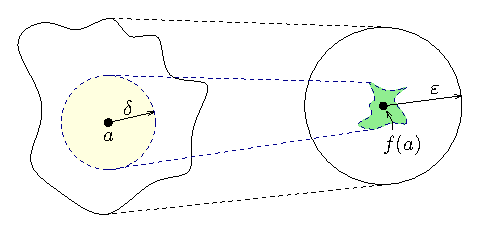
\includegraphics[width=0.5\textwidth]{10_3.eps}
		\caption{Открытый прообраз $\Rightarrow$ непрерывность.}
		\label{10_3}
	\end{figure}

	$(\Rightarrow)$	Пусть $V \subset Y$ - открытое множество, возьмем его прообраз $f^{-1}(V) = \{\,x \in X \mid f(x) \in V \,\}$. Рассмотрим точку $a \in f^{-1}(V)$ этого множества  $\Rightarrow$ по определению $\exists \, f(a) \in V$.
	\begin{figure}[H]
		\centering
		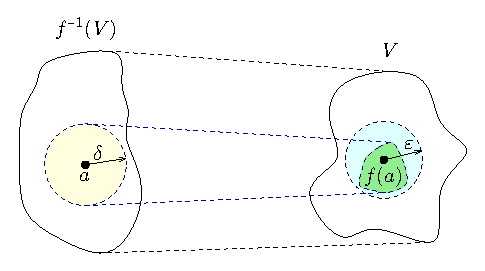
\includegraphics[width=0.5\textwidth]{10_4.eps}
		\caption{Непрерывность $\Rightarrow$ открытый прообраз.}
		\label{10_4}
	\end{figure}
	Поскольку $V \subset Y$ - открытое множество $\Rightarrow \exists \, B(f(a),\VE) \subset V$. По определению непрерывности: 
	$$
		\exists \, \delta > 0 \colon \rho_X(a,x) < \delta \Rightarrow \rho_Y(f(x),f(a)) < \VE
	$$
	это означает, что $f\big(B(a,\delta)\big) \subset B(f(a),\VE) \Rightarrow B(a,\delta) \subset f^{-1}\big(B(f(a),\VE)\big) \Rightarrow B(a,\delta)\subset f^{-1}(V)$. 
\end{proof}
\begin{exrc}
	Доказать, что:
	\begin{enumerate}[label ={(\arabic*)}]
		\item $f^{-1}(A \cup B) = f^{-1}(A) \cup f^{-1}(B)$;
		\item $f^{-1}(A \cap B) = f^{-1}(A) \cap f^{-1}(B)$;
		\item $f^{-1}(A \setminus B) = f^{-1}(A) \setminus f^{-1}(B)$;
		\item $\textstyle f^{-1}\Big(\bigcup\limits_{\alpha \smallin \MI}\MU_\alpha\Big) = \textstyle \bigcup\limits_{\alpha \smallin \MI}f^{-1}(\MU_\alpha)$;
		\item $\textstyle f^{-1}\Big(\bigcap\limits_{\alpha \smallin \MI}\MU_\alpha\Big) = \textstyle \bigcap\limits_{\alpha \smallin \MI}f^{-1}(\MU_\alpha)$;
	\end{enumerate}
\end{exrc}
\begin{proof}\hfill
	\begin{enumerate}[label ={(\arabic*)}]
		\item Пусть $x \in f^{-1}(A \cup B) \Leftrightarrow f(x) \in A \cup B \Leftrightarrow f(x) \in A \vee f(x) \in B \Leftrightarrow x \in f^{-1}(A) \vee x \in f^{-1}(B)\Leftrightarrow$\\  $\Leftrightarrow x \in  f^{-1}(A) \cup f^{-1}(B) \Rightarrow f^{-1}(A \cup B) = f^{-1}(A) \cup f^{-1}(B)$;
		\item Пусть $x \in f^{-1}(A \cap B) \Leftrightarrow f(x) \in A \cap B \Leftrightarrow f(x) \in A \wedge f(x) \in B \Leftrightarrow x \in f^{-1}(A) \wedge x \in f^{-1}(B)\Leftrightarrow$\\  $\Leftrightarrow x \in  f^{-1}(A) \cap f^{-1}(B) \Rightarrow f^{-1}(A \cap B) = f^{-1}(A) \cap f^{-1}(B)$;
		\item Пусть $x \in f^{-1}(A \setminus B) \Leftrightarrow f(x) \in A \setminus B \Leftrightarrow f(x) \in A \wedge f(x) \notin B \Leftrightarrow x \in f^{-1}(A)\wedge x \notin f^{-1}(B)\Leftrightarrow$\\ $\Leftrightarrow x \in f^{-1}(A) \setminus f^{-1}(B) \Rightarrow f^{-1}(A \setminus B) = f^{-1}(A) \setminus f^{-1}(B)$;
		\item Пусть $x \in f^{-1}\Big(\bigcup\limits_{\alpha \smallin \MI}\MU_\alpha\Big) \Leftrightarrow f(x) \in \bigcup\limits_{\alpha \smallin \MI}\MU_\alpha \Leftrightarrow \exists \, \alpha \in \MI \colon f(x) \in \MU_{\alpha} \Leftrightarrow \exists \, \alpha \in \MI \colon x \in f^{-1}(\MU_{\alpha}) \Leftrightarrow$\\
		$\Leftrightarrow x \in \textstyle \bigcup\limits_{\alpha \smallin \MI}f^{-1}(\MU_\alpha) \Rightarrow \textstyle f^{-1}\Big(\bigcup\limits_{\alpha \smallin \MI}\MU_\alpha\Big) = \textstyle \bigcup\limits_{\alpha \smallin \MI}f^{-1}(\MU_\alpha)$;
		\item Пусть $x \in f^{-1}\Big(\bigcap\limits_{\alpha \smallin \MI}\MU_\alpha\Big) \Leftrightarrow f(x) \in \bigcap\limits_{\alpha \smallin \MI}\MU_\alpha \Leftrightarrow \forall \alpha \in \MI,\, f(x) \in \MU_{\alpha} \Leftrightarrow \forall \alpha \in \MI,\, x \in f^{-1}(\MU_{\alpha}) \Leftrightarrow$\\
		$\Leftrightarrow x \in \textstyle \bigcap\limits_{\alpha \smallin \MI}f^{-1}(\MU_\alpha) \Rightarrow \textstyle f^{-1}\Big(\bigcap\limits_{\alpha \smallin \MI}\MU_\alpha\Big) = \textstyle \bigcap\limits_{\alpha \smallin \MI}f^{-1}(\MU_\alpha)$;
	\end{enumerate}
\end{proof}
\begin{exrc}
	Верно ли, что $f \colon X \to Y$ - непрерывно $\Leftrightarrow$ прообраз замкнутого множества - замкнут.
\end{exrc}
\begin{proof}
	$(\Rightarrow)$ Пусть $f$ - непрерывно, $V \subset Y$ - замкнуто $\Rightarrow Y \setminus V$ - открыто $\Rightarrow f^{-1}(Y\setminus V)$ - тоже открыто по теореме выше $\Rightarrow f^{-1}(Y\setminus V) = f^{-1}(Y)\setminus f^{-1}(V)$ - открыто. По определению $f^{-1}(Y) = X \Rightarrow X \setminus f^{-1}(V)$ - открыто $\Rightarrow f^{-1}(V)$ - замкнутое множество.
	
	$(\Leftarrow)$ Пусть $\forall$ замкнутого множества $V \subset Y$, его прообраз $f^{-1}(V)$ - тоже замкнут. Пусть $U \subset Y$ - открытое множество $\Rightarrow Y\setminus U$ - замкнуто $\Rightarrow f^{-1}(Y \setminus U ) = f^{-1}(Y)\setminus f^{-1}(U) = X \setminus f^{-1}(U)$ - замкнутое множество $\Rightarrow f^{-1}(U)$ - открытое множество, таким образом любое прообраз открытого множества - открытое множество $\Rightarrow$ по теореме выше функция $f$ - непрерывная.
\end{proof}

\begin{corollary}
	Пусть $(X,\rho_X),\, (Y,\rho_Y)$ - метрические пространства. Если $f \colon X \to Y$ - непрерывная функция и множество $K \subset X$ - компакт, то $f(K)$ - компакт.
\end{corollary}
\begin{rem}
	Обратное утверждение не верно, смотри, например, функцию Дирихле (отображает всё в две точки, две точки это всегда компакт).
\end{rem}
\begin{proof}
	Пусть $f(K) \subset \textstyle \bigcup\limits_{\alpha} \MU_\alpha$, где $\MU_\alpha$ - открыты. Пусть $x \in K$, тогда:
	$$
		 f(x) \in \textstyle \bigcup\limits_{\alpha} \MU_\alpha \Rightarrow x \in f^{-1}\Big(\textstyle \bigcup\limits_{\alpha} \MU_\alpha\Big)
	$$ 
	Таким образом $K \subset \textstyle f^{-1}\Big(\bigcup\limits_{\alpha}\MU_\alpha\Big) = \textstyle \bigcup\limits_{\alpha}f^{-1}(\MU_\alpha)$. Прообразы открытых множеств - открыты, а $K$ - компакт, тогда: 
	$$
		\exists \, \alpha_1,\dotsc \alpha_N \colon K \subset f^{-1}(\MU_{\alpha_1})\cup \dotsc \cup f^{-1}(\MU_{\alpha_N}) = f^{-1}(\MU_{\alpha_1} \cup \dotsc \cup \MU_{\alpha_N})
	$$ 
	Пусть $x \in K \Rightarrow x \in f^{-1}(\MU_{\alpha_1} \cup \dotsc \cup \MU_{\alpha_N})$, тогда по определению: 
	$$
		\forall x \in K \Rightarrow x \in f^{-1}(\MU_{\alpha_1} \cup \dotsc \cup \MU_{\alpha_N}) \Rightarrow f(x) \in \MU_{\alpha_1} \cup \dotsc \cup \MU_{\alpha_N} \Rightarrow f(K) \subset \MU_{\alpha_1} \cup \dotsc \cup \MU_{\alpha_N}
	$$
	Таким образом $f(K)$ - компакт.
\end{proof}
\begin{exrc}
	Пусть $f \colon X \to Y$ - непрерывна, верно ли что:
	\begin{enumerate}[label ={(\arabic*)}]
		\item Образ ограниченного множества является ограниченным множеством;
		\item Образ замкнутого множества является замкнутым множеством;
	\end{enumerate}
\end{exrc}
\begin{proof}\hfill
	\begin{enumerate}[label ={(\arabic*)}]
		\item Рассмотрим функцию $f(x) = \tfrac{1}{x},\, V = (0,1]$ - ограниченное множество, но $f(V) = [1, +\infty)$ - не является ограниченным множеством;	
		\item Рассмотрим функцию $f(x) = \tfrac{1}{1+x^2} \Rightarrow V = \MR$ - замкнутое множество, но $f(V) = (0,1]$ - не является замкнутым множеством;
	\end{enumerate}
\end{proof}

\begin{corollary}
	\textbf{(Теорема Вейрштрасса)}: Пусть $K$ - компакт и $f \colon K \to \MR$ - непрерывная функция. Тогда $f$ - ограничена и $\exists\, x_m, x_M \in K$: 
	$$
		f(x_m) = \inf\limits_{K}f(x), \, f(x_M) = \sup\limits_{K}f(x)
	$$
\end{corollary}
\begin{proof}
	$f(K)$ - компакт в $\MR$, то есть ограниченное и замкнутое множество. По определению точной верхней грани 
	$$
		\forall y \in f(K) \colon \sup\limits_{K}f(x) \geq y \Rightarrow \forall z \in \MR \colon z > \sup\limits_{K}f(x) \Rightarrow z \notin f(K)
	$$ 
	С другой стороны, точная верхняя грань - самая маленькая среди всех верхних граней, тогда $$
		\forall \VE > 0, \, \exists \, y \in f(K) \colon (\sup\limits_{K}f(x) - \VE) < y
	$$ 
	иначе нашелся бы $\VE_0$ такой, что $\forall y \in f(K), \, y \leq (\sup\limits_{K}f(x) - \VE_0) < \sup\limits_{K}f(x) \Rightarrow (\sup\limits_{K}f(x) - \VE_0)$ - точная верхняя грань и получили бы противоречие. Аналогичные рассуждения справделивы для точной нижней грани. Таким образом, какую бы окрестность точной грани не взяли, то в ней всегда будут как точки из множества $f(K)$, так и точки не из этого множества $\Rightarrow$ это граничные точки.
	
	Так как $\inf\limits_{K}f, \, \sup\limits_{K}f$ - граничные точки $f(K)$, то они принадлежат $f(K) \Rightarrow \exists\, x_m, x_M \in K$:
	$$
		f(x_m) = \inf\limits_{K}f(x), \, f(x_M) = \sup\limits_{K}f(x)
	$$
\end{proof}
\begin{theorem}
	\textbf{(Кантора)}: Пусть $K$ - компакт, $Y$ - метрическое пространство. Если $f\colon K \to Y$ - непрерывна. Тогда $f$ - равномерно непрерывна, то есть:
	$$
		\forall \VE > 0, \, \exists \, \delta > 0 \colon \forall x,y \in K, \, \rho_K(x,y) < \delta \Rightarrow \rho_Y(f(x),f(y)) < \VE 
	$$
\end{theorem}
\begin{proof}\hfill\\
	\textbf{(\RN{1}) способ}: (От противного) Пусть $f$ - непрерывно, но не является равномерно непрерывной, тогда:
	$$
		\exists \, \VE > 0, \, \forall \delta > 0 \colon \exists \, x,y \in K, \rho_K(x,y) < \delta  \wedge \rho_Y(f(x),f(y)) \geq \VE > 0
	$$
	Пусть $\delta = \dfrac{1}{n}, \, x_n, y_n \in K \colon \rho_K(x_n,y_n) < \dfrac{1}{n}$. Так как $K$ - компакт, то $\exists \, x_{n_k} \to x_0 \in K \Rightarrow y_{n_k} \to x_0$. По непрерывности $f(x_{n_k}) \to f(x_0) \wedge f(y_{n_k}) \to f(x_0) \Rightarrow 0 < \VE \leq \rho_Y(f(x_{n_k}),f(y_{n_k})) \to 0 \Rightarrow$ противоречие.
	
	\textbf{(\RN{2}) способ}: Пусть $\VE >0$, тогда по непрерывности функции $f$ получим:
	$$
		\forall a \in K, \, \exists \, B(a,\delta_a) \colon \forall x,y \in B(a,\delta_a), \, \rho_Y(f(x),f(a)) < \frac{\VE}{2},\, \rho_Y(f(y),f(a)) < \frac{\VE}{2} \Rightarrow \rho_Y(f(x),f(y)) < \VE
	$$
	Очевидно, что компакт есть подмножество $K \subset \textstyle \bigcup\limits_{a \smallin K}B\big(a,\tfrac{\delta_a}{3}\big)$. Из-за компактности $\exists$ конечное подпокрытие $K$: $B\big(a_1,\tfrac{\delta_{a_1}}{3}\big), \dotsc, B\big(a_N,\tfrac{\delta_{a_N}}{3}\big)$. Пусть $\delta = \min\{\tfrac{\delta_{a_1}}{3}, \dotsc, \tfrac{\delta_{a_N}}{3}\}$. Пусть $\rho_K(x,y) < \delta$, поскольку компакт покрыт, то $\exists \, B\big(a_j,\tfrac{\delta_{a_j}}{3}\big) \colon x \in B\big(a_j,\tfrac{\delta_{a_j}}{3}\big)$, тогда:
	$$
		\rho_K(y,a_j) \leq \rho_K(y,x)  + \rho_K(x,a_j) < \dfrac{2\delta_{a_j}}{3} \Rightarrow x,y \in B(a_j, \delta_{a_j}) \Rightarrow \rho_Y(f(x),f(y)) < \VE
	$$
	Таким образом, мы нашли $\delta > 0$ такой, что:
	$$
		\forall \VE > 0, \, \exists \, \delta > 0 \colon \forall x,y \in K, \, \rho_K(x,y) < \delta \Rightarrow \rho_Y(f(x),f(y)) < \VE 
	$$
\end{proof}


\newpage
\section*{Связные множества в метрическом пространстве}
\begin{defn}
	Метрическое пространство $(X,\rho)$ \uwave{несвязно}, если существуют непустые открытые множества $U,V \colon U \cap V = \VN \wedge X = U \cup V$.
\end{defn}

\begin{figure}[H]
	\centering
	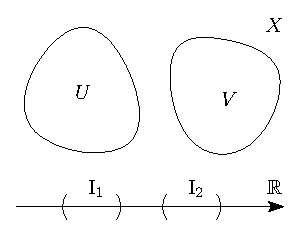
\includegraphics[width=0.3\textwidth]{10_5.eps}
	\caption{Неcвязные множества: метрическое пространство $X = U \cup V$; на $\MR$ - интервалы $\mathrm{I}_1$ и  $\mathrm{I}_2$.}
	\label{10_5}
\end{figure}

\begin{defn}
	Множество $E$ в метрическом пространстве $(X,\rho)$ \uwave{несвязно}, если существуют открытые множества $U,V \colon E \cap U \neq \VN$, $E \cap V \neq \VN$, $U \cap V = \VN$ и $E \subset U \cup V$.
\end{defn}
\begin{figure}[H]
	\centering
	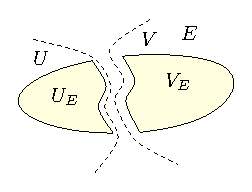
\includegraphics[width=0.3\textwidth]{10_6.eps}
	\caption{Неcвязные множества можно разделить открытыми множествами}
	\label{10_6}
\end{figure}
Пусть $E \subset X$ несвязно в $E$, будет ли оно также несвязно при продолжении на пространство $X$? Вдруг множество $E = U \cup V$ несвязно, но как ни дополнишь до метрического пространства, множества $U$ и $V$ будут пересекаться?
 
\begin{figure}[H]
	\centering
	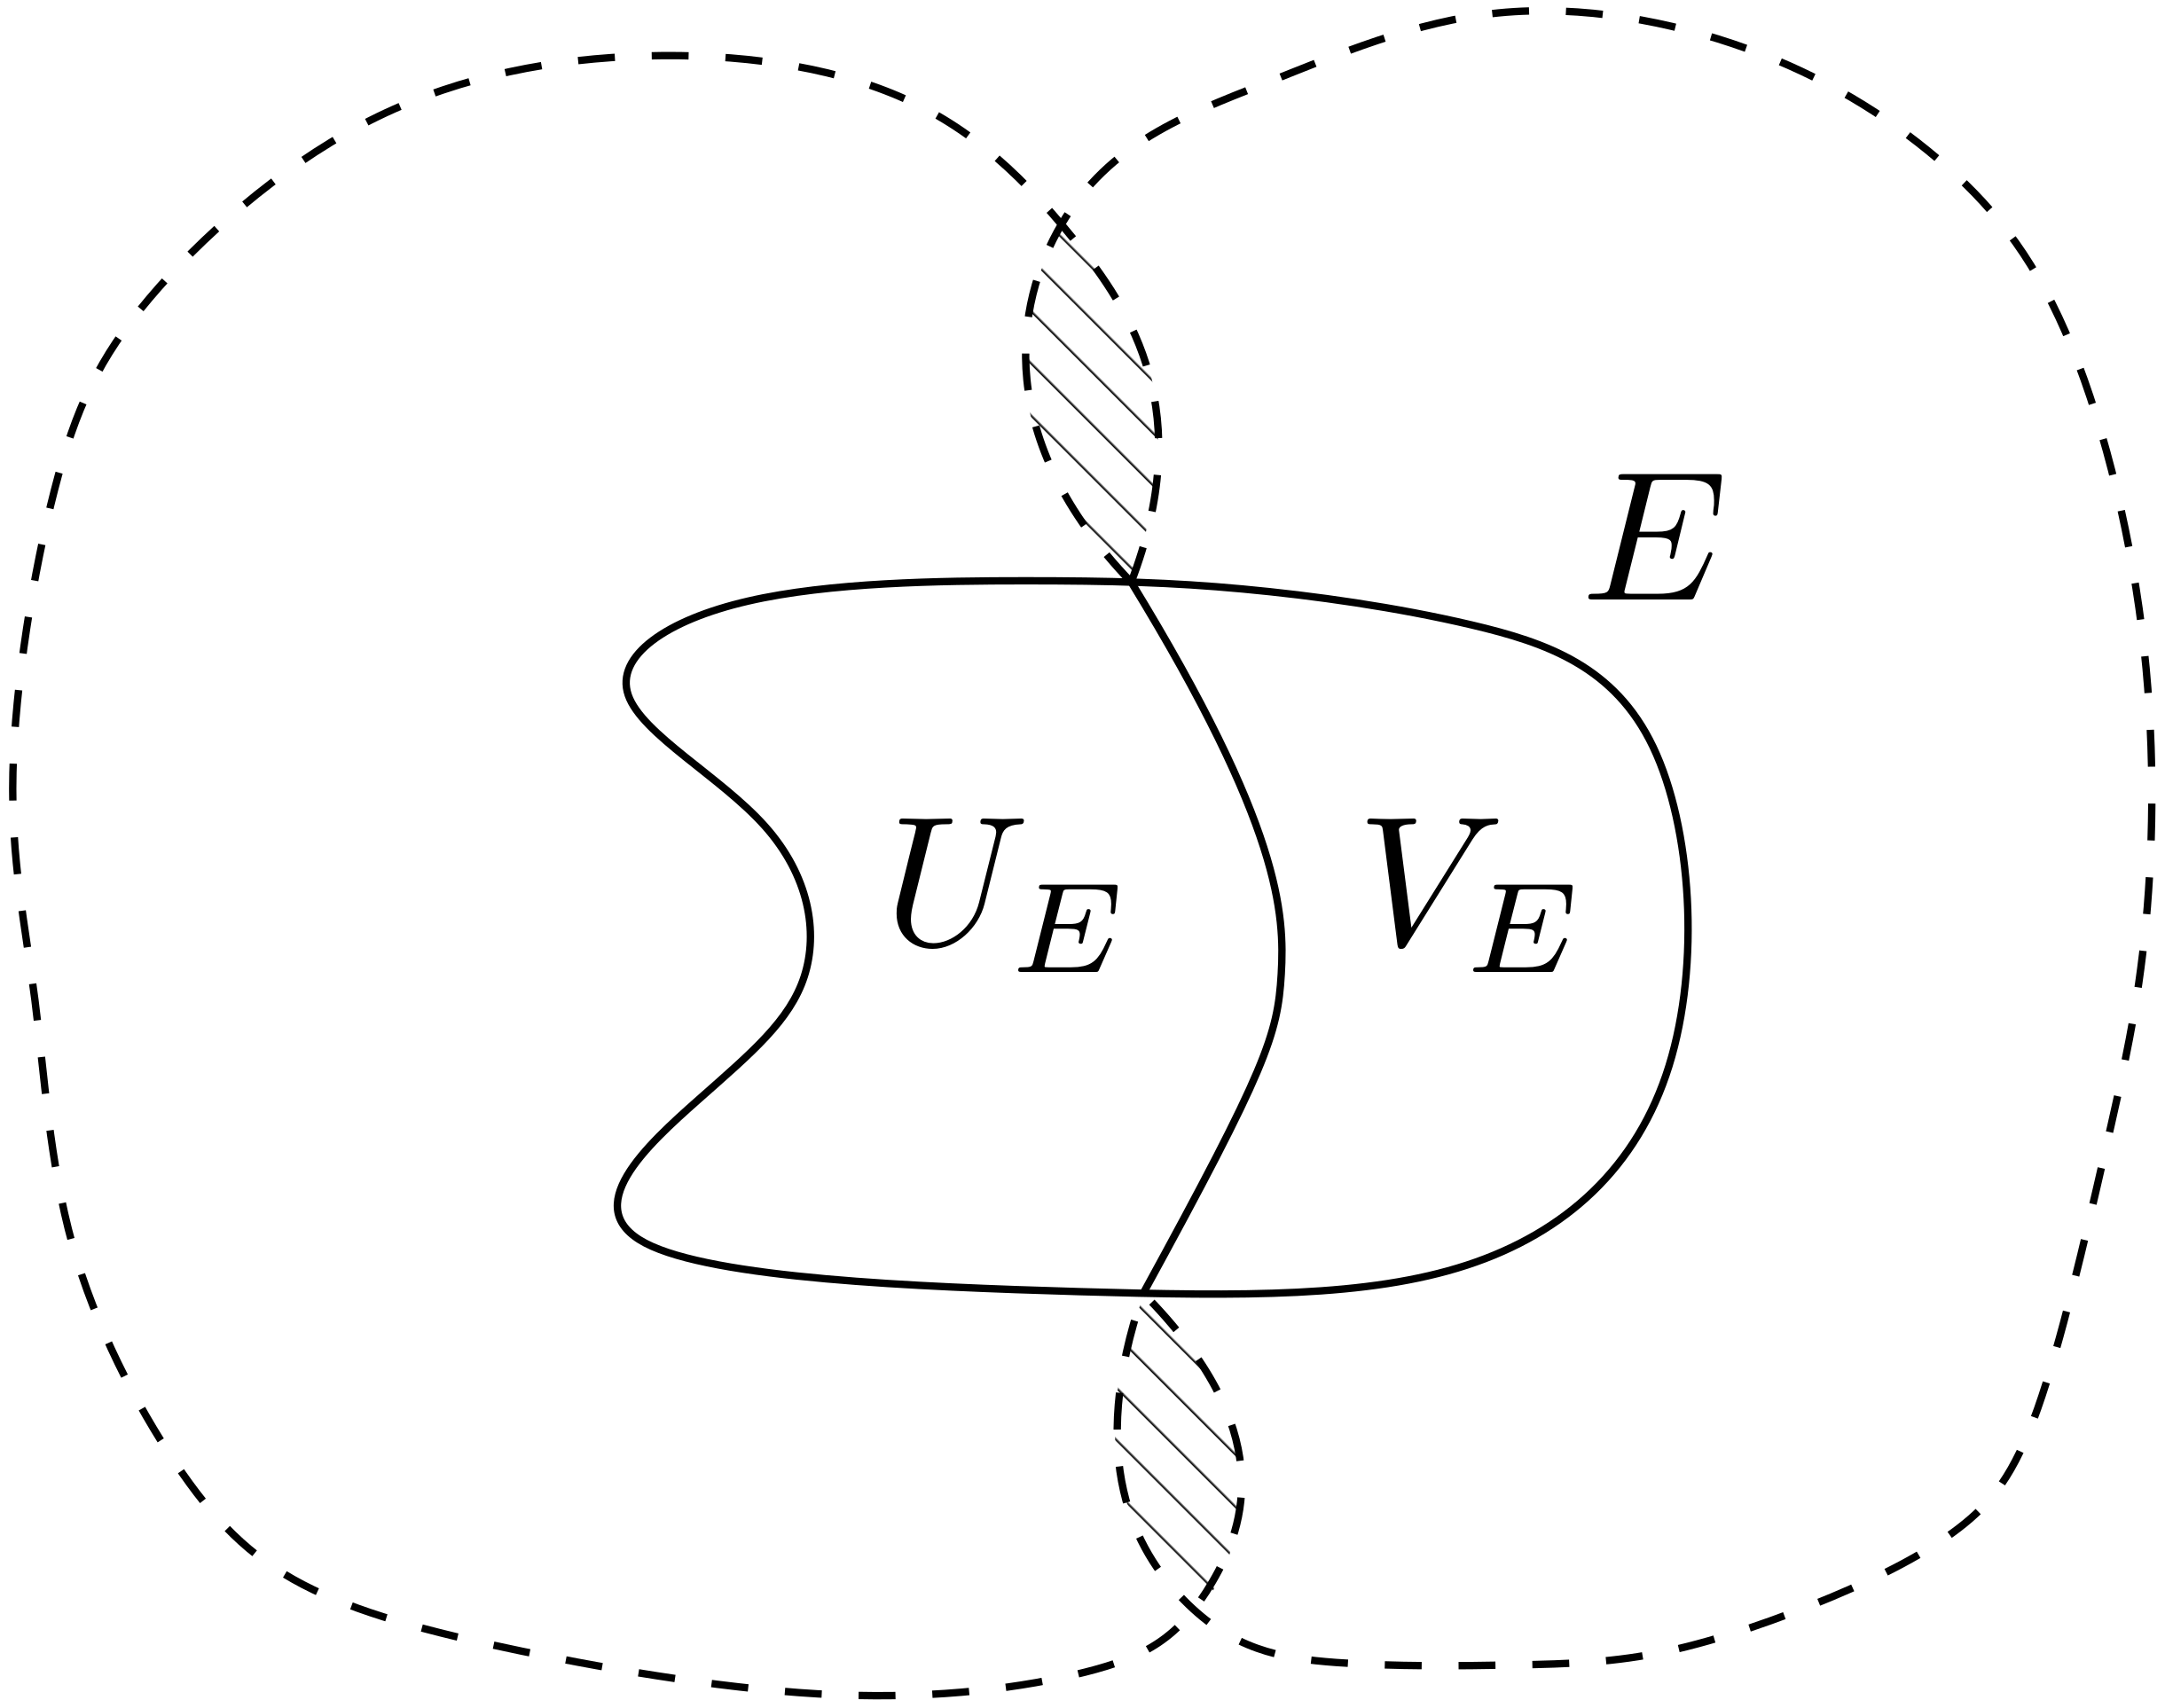
\includegraphics[width=0.3\textwidth]{10_7.png}
	\caption{Неcвязное множество $E$ несвязно в $(E,\rho) \Rightarrow$ несвязно в $(X,\rho)$?}
	\label{10_7}
\end{figure}

На самом деле такая ситуация невозможна и ответ на этот вопрос дает следующая теорема.

\begin{theorem}
	Пусть $(X,\rho)$ - метрическое пространство. $E \subset X$ несвязно $\Leftrightarrow E$  несвязно в метрическом пространстве $(E,\rho)$.
\end{theorem}

\begin{proof}\hfill\\
	$(\Rightarrow)$ Если $\exists$ открытые $U, V$ такие, что: 
	$$
		U \cap V = \VN, \, E \cap U \neq \VN, \,E \cap V \neq \VN, \, E \subset U \cup V
	$$ 
	то $U_E = U \cap E, \, V_E = V \cap E$ - открыты в $E$, непусты, $U_E \cap V_E = \VN$ и $E = U_E \cup V_E$.
	
	$(\Leftarrow)$ Пусть $E = U_E \cup V_E$, где $U_E, V_E$ - открыты и непусты в $E$ и $U_E \cap V_E = \VN$. Тогда, в каждом из множеств можно взять точку и некоторую окрестность вокруг неё: 
	$$
		\forall a \in U_E, \, \exists \, B(a,\delta_a) \colon B(a,\delta_a) \cap E \subset U_E \wedge \big(B(a,\delta_a)\cap E \big) \cap V_E = \VN
	$$ 
	$$
		\forall b \in V_E, \, \exists \, B(b,\delta_b) \colon B(b,\delta_b) \cap E \subset V_E \wedge \big(B(b,\delta_b)\cap E \big) \cap U_E = \VN
	$$ 
	
	Рассмотрим множества: 
	$$
		U = \textstyle \bigcup\limits_{a \smallin U_E}B\big(a, \tfrac{\delta_a}{2}\big), \, V = \textstyle \bigcup\limits_{a \smallin V_E}B\big(b, \tfrac{\delta_b}{2}\big)
	$$ 
	проверим, что $U \cap V = \VN$. Пусть это не так и $\exists \, x \in U \cap V$, тогда 
	$$
		\exists \, a \in U_E, \, b \in V_E \colon x \in B\big(a,\tfrac{\delta_a}{2}\big)\wedge x \in B\big(b,\tfrac{\delta_b}{2}\big)
	$$
	Это ознчает, что
	
	$$
		\rho(a,x) < \frac{\delta_a}{2} \wedge \rho(b,x) < \frac{\delta_b}{2} \Rightarrow \rho(a,b) < \frac{\delta_a + \delta_b}{2} < \max\{\delta_a,\delta_b\}
	$$
	Пусть $\delta_a \geq \delta_b \Rightarrow \rho(a,b) < \delta_a \Rightarrow b \in B(a,\delta_a) \Rightarrow$ так как $b \in V_E$, но $\big(B(a,\delta_a)\cap E \big) \cap V_E = \VN$, то получаем противоречие. Получили, что  $U \cap V = \VN$.
	
	Остальные свойства очевидно выполнены: $E \cap U \neq \VN, \,E \cap V \neq \VN, \, E \subset U \cup V$.
\end{proof}
\end{document}